\documentclass[landscape,a0b,final,a4resizeable]{a0poster}
%\documentclass[landscape,a0b,final]{a0poster}
%\documentclass[portrait,a0b,final,a4resizeable]{a0poster}
%\documentclass[portrait,a0b,final]{a0poster}
%%% Option "a4resizeable" makes it possible ot resize the
%   poster by the command: psresize -pa4 poster.ps poster-a4.ps
%   For final printing, please remove option "a4resizeable" !!

\usepackage{amsmath}
\usepackage{amssymb}
\usepackage{bm}
\usepackage{multicol}
\usepackage{multirow}
\usepackage[usenames,dvipsnames]{color}
\usepackage{psfrag}
\usepackage{epsfig}
\usepackage{subfigure}
\usepackage{pstricks,pst-grad,calc}
\usepackage{algorithmic}
\usepackage{algorithm}
\usepackage{enumerate}
\usepackage{tikz}
\usetikzlibrary{arrows,shapes,snakes,automata,backgrounds,fit,petri}

% Definitions
\setlength{\columnsep}{3cm}
\setlength{\columnseprule}{2mm}
\setlength{\parindent}{0.0cm}

% Background
\newcommand{\background}[3]{
	\newrgbcolor{cbegin}{#1}
	\newrgbcolor{cend}{#2}
	\psframe[fillstyle=gradient, gradlines=1000, gradend=cend, gradbegin=cbegin,
           	 gradangle=0, gradmidpoint=#3]( 0., 0. )( 1.\textwidth, -1.\textheight )
}

% Poster environment
\newenvironment{poster}{
	\begin{center} \begin{minipage}[c]{0.98\textwidth} }{
	\end{minipage} \end{center}
}

% Custom column
\newenvironment{pcolumn}[1]{
	\begin{minipage}{#1\textwidth} \begin{center} }{
  	\end{center} \end{minipage}
}

% Custom box
\newcommand{\pbox}[4]{
	\psshadowbox[#3]{
		\begin{minipage}[t][#2][t]{#1}
			#4
		\end{minipage}
}}

% Custom section
\newcommand{\csection}[1]{
\vspace{0.1cm}
\begin{center}
	\pbox{0.8\columnwidth}{}{linewidth=2mm, framearc=0.0, linecolor=lightgreen, fillstyle=gradient,
	                         gradangle=0, gradbegin=white, gradend=whitegreen, gradmidpoint=1.0, framesep=0.6em, shadowsize=0
	                        }{\begin{center}{\bf \large #1}\end{center}}
\end{center}
\vspace{0.1cm}
}

% Custom caption
\setcounter{figure}{1}
\setcounter{table}{1}

\newcommand{\tcaption}[1]{
  \vspace{0.3cm}
  \begin{quote}
    {{\sc Table} \arabic{table}: #1}
  \end{quote}
  %\vspace{0.3cm}
  \stepcounter{table}
}

\newcommand{\fcaption}[1]{
  \vspace{0.3cm}
  \begin{quote}
	\centering
    {{\sc Figure} \arabic{figure}: \small {#1}}
  \end{quote}
  \vspace{0.6cm}
  \stepcounter{figure}
}

\renewcommand\refname{ }

% Math definitions
%
% Useful definitions for vectors and stuff
%

% matrices and vectors
\def\A{{\bf A}}
\def\a{{\bf a}}
\def\B{{\bf B}}
\def\b{{\bf b}}
\def\C{{\bf C}}

\def\D{{\bf D}}
\def\E{{\bf E}}
\def\e{{\bf e}}

\def\F{{\bf F}}
\def\f{{\bf f}}
\def\G{{\bf G}}
\def\g{{\bf g}}
\def\H{{\bf H}}
\def\h{{\bf h}}
\def\I{{\bf I}}



\def\K{{\bf K}}
\def\k{{\bf k}}
\def\L{{\bf L}}

\def\M{{\bf M}}
\def\m{{\bf m}}




\def\P{{\bf P}}

\def\Q{{\bf Q}}
\def\q{{\bf q}}
\def\R{{\bf R}}
\def\r{{\bf r}}
\def\S{{\bf S}}
\def\s{{\bf s}}
\def\t{{\bf t}}
\def\U{{\bf U}}
\def\u{{\bf u}}
\def\V{{\bf V}}
\def\v{{\bf v}}
\def\W{{\bf W}}
\def\w{{\bf w}}
\def\X{{\bf X}}
\def\x{{\bf x}}
\def\Y{{\bf Y}}
\def\y{{\bf y}}
\def\Z{{\bf Z}}
\def\z{{\bf z}}

% permutations
\def\PL{{\bf P}_\mathrm{r}}
\def\PR{{\bf P}_\mathrm{c}}
\def\PC{{\bf P}_\mathrm{f}}

% more stuff
\def\BNet{{\cal B}}
\def\GR{{\cal D}}
\def\ED{{\cal E}}
% \def\S{{\cal S}}
\def\VR{{\cal V}}
\def\Sp{{\cal S}}
\def\0{{\bf 0}}
\def\1{{\bf 1}}

\def\Re{\mathbb{R}}
\def\Ex{\mathbb{E}}
\def\Lik{\mathcal{L}}

\def\<{\, \langle \,}
\def\>{\, \rangle \,}
\def\inv{^{-1}}
\def\ts{^\top}
\def\lik{{\cal L}}
\def\topc{\mathrm{top}}

% mathrms
\def\sign{\mathrm{sign}}
\def\max{\mathrm{max}}
\def\min{\mathrm{min}}
\def\tr{\mathrm{trace}}
\def\diag{\mathrm{diag}}
\def\MAP{\mathrm{MAP}}
\def\ICA{\mathrm{ICA}}
\def\FM{\mathrm{FM}}
\def\DAG{\mathrm{DAG}}
\def\FA{\mathrm{FA}}
\def\BN{\mathrm{BN}}
\def\rep{\mathrm{rep}}
\def\block{\mathrm{block}}
\def\abs{\mathrm{abs}}

% bold greeks
\def\balpha{\bm{\alpha}}
\def\bbeta{\bm{\beta}}
\def\bPsi{\bm{\Psi}}
\def\bSigma{\bm{\Sigma}}
\def\bepsilon{\bm{\epsilon}}
\def\bupsilon{\bm{\upsilon}}
\def\bmeta{\bm{\eta}}
\def\bmu{\bm{\mu}}
\def\bnu{\bm{\nu}}
\def\btau{\bm{\tau}}
\def\bLambda{\bm{\Lambda}}
\def\bTheta{\bm{\Theta}}

% distributions
\def\DN{\mathcal{N}}
\def\TN{\mathcal{TN}}
\def\IG{\mathrm{IG}}
\def\La{\mathrm{Laplace}}
\def\Exp{\mathrm{Exponential}}
\def\Uni{\mathrm{Uniform}}
\def\Be{\mathrm{Beta}}
\def\Bin{\mathrm{Binomial}}
\def\Ber{\mathrm{Bernoulli}}
\def\Ga{\mathrm{Gamma}}
\def\Poi{\mathrm{Poisson}}
\def\GP{\mathrm{GP}}
\def\DP{\mathrm{DP}}
\def\TP{\mathrm{TP}}
\def\IGamma{{\cal IG}}
\def\DGamma{{\cal G}}
\def\Wish{\mathrm{Wishart}}
\def\IW{{\cal IW}}
\def\MOD{\mathcal{M}}
\def\LN{\mathrm{logNormal}}

% commands
\newcommand{\argmax}{\operatornamewithlimits{argmax}}
\newcommand{\argmin}{\operatornamewithlimits{argmin}}
\newcommand{\deff}{\overset{\underset{\mathrm{def}}{}}{=}}
\newcommand{\indi}{\overset{\underset{\mathrm{ind}}{}}{\sim}}
\newcommand{\Perp}{\perp \! \! \! \perp}

\newcommand{\ie}{i.e. }
\newcommand{\eg}{e.g. }
\newcommand{\wrt}{w.r.t. }
\newcommand{\iid}{i.i.d. }

\newcommand{\tmp}[1]{{\color{orange} {\bf #1}}}
\newcommand{\quotes}[1]{``#1''}

\def\ctilde{\kern -.04em\lower .7ex\hbox{\~{}}\kern .04em}

\def\Tiny{\fontsize{5pt}{5pt}\selectfont}


\begin{document}

\background{1.0 1.0 1.0}{1.0 1.0 1.0}{1.0}
\vspace*{1cm}

\newrgbcolor{lightblue}{0. 0. 0.80}
\newrgbcolor{white}{0.988 1.000 0.960}
\newrgbcolor{whiteblue}{.80 .80 1.}
\newrgbcolor{lightgreen}{0.349 0.376 0.431}
\newrgbcolor{whitegreen}{0.678 0.658 0.580}

\begin{poster}
%
\begin{center}
\begin{pcolumn}{0.99}
%
\pbox{0.95\textwidth}{}{linewidth=2mm, framearc=0.0, linecolor=lightgreen, fillstyle=gradient,
                        gradangle=0,gradbegin=white,gradend=whitegreen,gradmidpoint=1.0,framesep=0.5em,shadowsize=0}
{
% University logo
\begin{minipage}[c][7cm][c]{0.1\textwidth}
	\begin{center}
    	
\includegraphics[width=12cm,angle=0]{images/dtu_logo}
	\end{center}
\end{minipage}
% Title and Authors
\begin{minipage}[c][7cm][c]{0.78\textwidth}
 	\begin{center}
    	{\huge {\bf Real-Time Rendering of Translucent Materials with Directional Subsurface Scattering} } \\ [10mm]
    	{\Large Alessandro Dal Corso - MSc Thesis} \\ [7.5mm]
			DTU Compute $\cdot$ Technical University of Denmark\\
			Lyngby, Denmark 
  	\end{center}
\end{minipage}
% Department logo
\begin{minipage}[c][7cm][c]{0.1\textwidth}
	\begin{center}
   		\includegraphics[width=12cm,angle=0]{images/dtucompute_logo}
	\end{center}
\end{minipage}
%
}
\end{pcolumn}
\end{center}
%
\vspace*{0.5cm}
%
\begin{multicols}{3}
%
\csection{Introduction}
%
\begin{itemize}
	\item We present a new BSSRDF Model in order to compute accurate subsurface scattering (SS) accounting for the direction of the incoming light.
	\item We explain an optimized GPU technique that enables rendering using the given model at interactive frame rates.
\end{itemize}
\vspace{-1cm}
%
\csection{Theory}
%
\vspace{-0.6cm}
{\bf BSSRDF function}
\vspace{0.6cm}

\emph{Subsurface scattering} (SS) is a physical phenomenon that naturally occurs in a wide range of natural materials. Some of the materials that exhibit a strong SS effect in everyday life are milk, human skin and marble. Subsurface scattering is that phenomenon that occurs when light is partially absorbed by an object, bounces inside ("scatters") and finally exits the surface on another point of the material.
\begin{center}
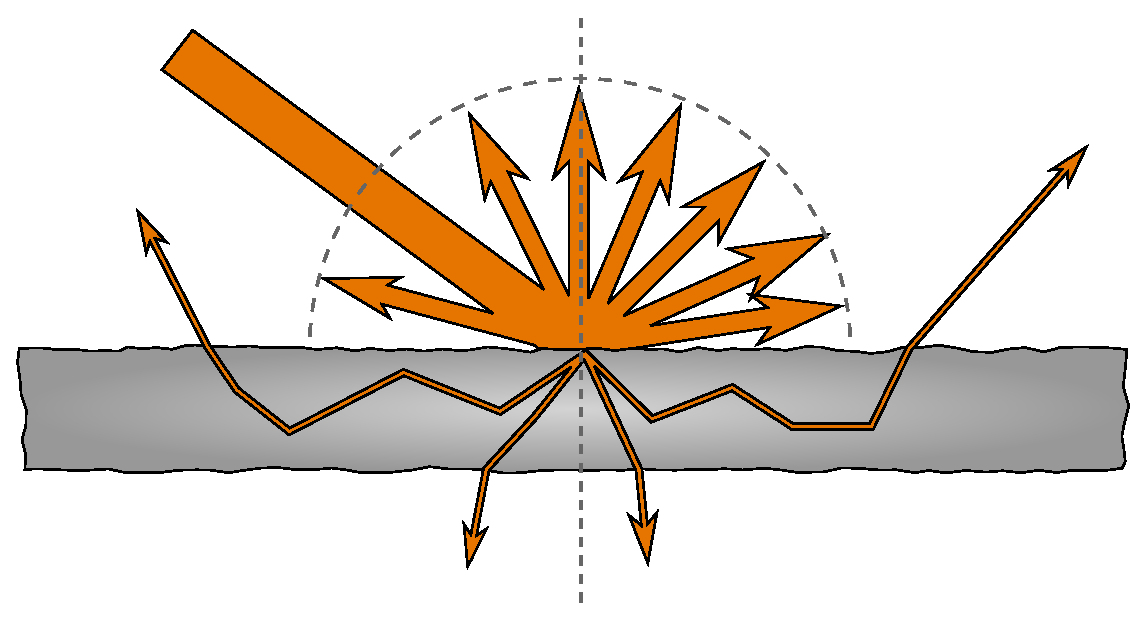
\includegraphics[scale = 1]{./images/diagram.eps} 
\fcaption{Diagram of subsurface scattering. Most of the incoming light gets reflected, but some of it enters the material and leaves it at a different point.}
\end{center}
In order to faithfully represent SS in computer graphics, we use a BSSRDF (\textit{Bidirectional surface scattering reflectance distribution function})\cite{Nicodemus:1992:GCN:136913.136929}, a function that describes how the light scatters within the medium. More precisely, a BSSRDF is a function $S$ between two points $\mathbf{x}_i$ and $\mathbf{x}_o$ on the surface that describes the ratio between an element of emergence radiance $dL(\mathbf{x}_o, \vec{\omega}_o)$ and an element of incident flux $d\Phi(\mathbf{x}_i,\vec{\omega}_i)$:

$$
S(\mathbf{x}_i, \vec{\omega}_i,\mathbf{x}_o, \vec{\omega}_o) = \frac{dL(\mathbf{x}_o, \vec{\omega}_o)}{d\Phi(\mathbf{x}_i,\vec{\omega}_i)}
$$

We can then use the BSSRDF in the general formulation of the rendering equation\cite{Jensen:2001:PMS:383259.383319}, obtaining:

\begin{equation}
\label{eq:eq1}
\begin{aligned}
L_o(\mathbf{x}_o, \vec{\omega}_o) &= L_e(\mathbf{x}_o, \vec{\omega}_o) + L_r(\mathbf{x}_o, \vec{\omega}_o) \\
&= L_e(\mathbf{x}_o, \vec{\omega}_o) + \int_A \int_{2\pi} S(\mathbf{x}_i, \vec{\omega}_i,\mathbf{x}_o, \vec{\omega}_o) L_i(\mathbf{x}_i, \vec{\omega}_i)(\vec{\omega}_i \cdot \vec{n}_i) d\vec{\omega}_i dA
\end{aligned}
\end{equation}

In order to obtain a good approximation for the BSSRDF functions, usually the BSSRDF term is split into two or more additional terms, accounting for single and multiple scattering. In case of multiple scattering, i.e. when light bounces multiple times inside the material, the radiance becomes largely isotropic, and the whole process can be treated as a diffusion process\cite{books/daglib/0093591}.  

\vspace{0.6cm}
{\bf Directional subsurface scattering}
\vspace{0.6cm}

In Jensen et al.\cite{Jensen:2001:PMS:383259.383319}, based on approximations of the diffusion equation, the BSSRDF $S$ is modeled as two points lights positioned close to $\mathbf{x}_i$, and depended on the distance between the points and the scattering parameters. In the model we are considering for our thesis\cite{IMM2013-06646}, proposed by Firsvad et al., we use a dipole of ray sources in order to better approximate the diffusion equation. The derived BSSRDF describes effectively the diffusion on an infinite medium, so some corrections are necessary in order to account for boundary conditions.

\begin{center}
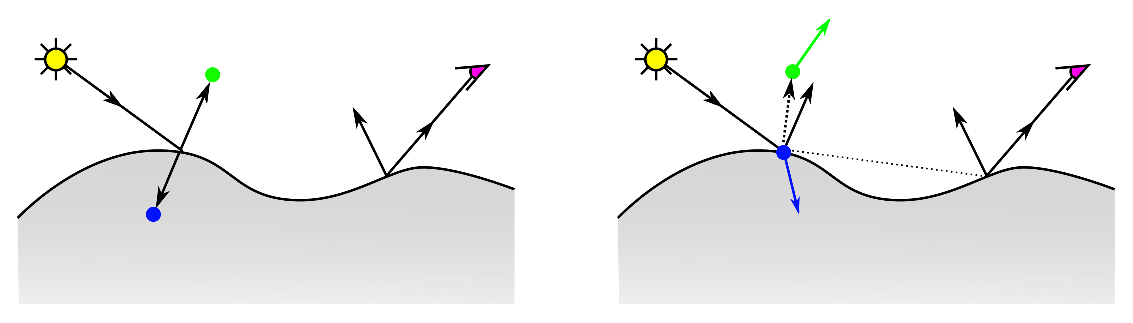
\includegraphics[scale = 1.4 ]{./images/comparison.eps} 
\fcaption{Standard dipole (on the left) versus directional dipole (on the right). }
\end{center}

%
\csection{Approximation}

The general idea of our  approach is to integrate Equation \ref{eq:eq1} numerically. In order to do this, we need to make some assumptions. Given an emergence point $\mathbf{x}_o$
\begin{itemize}
  \item We limit to directional lights (but we can extend this method later to other kind of lights).
	\item Only the points within a certain \emph{projected radius} contribute to the emitted radiance.
	\item Each of the considered points covers the same area element. 
\end{itemize}

Given these assumptions, the radiance of the incoming light $L_i$becomes a constant. Discretizing the integral and considering not emitting bodies, we obtain:

\begin{equation}
L_o(\mathbf{x}_o, \vec{\omega}_o) = L_i \sum_{i = 0}^{k} S(\mathbf{x}_i, \vec{\omega}_i,\mathbf{x}_o, \vec{\omega}_o) (\vec{\omega}_i \cdot \vec{n}_i) A_k
\label{eq:2}
\end{equation}

Where $k$ is the number of samples, and $A_k$ is the area element. $A_k$ is equal of the average area of a sample divided by the projection term: $\frac{A_{circle}}{k \vec{\omega}_i \cdot \vec{n}_i}$. Inserting into Equation \ref{eq:2} we obtain the final approximation: 

\begin{equation}
L_o(\mathbf{x}_o, \vec{\omega}_o) = L_i \frac{A_{circle}}{k} \sum_{i = 0}^{k} S(\mathbf{x}_i, \vec{\omega}_i,\mathbf{x}_o, \vec{\omega}_o)
\label{eq:3}
\end{equation}
\vspace{-1cm}
\csection{Implementation}
\vspace{-1cm}
In order to implement the approximation in Equation \ref{eq:3}, we employ a four pass technique that requires only the pure object model, without the necessity of a uv mapping. Since the computation of the BSSRDF is expensive, we split it into subsequent frames, continuously improving the result until convergence. The technique is inspired from translucent shadow maps, with some changes in order to adapt to the particular BSSRDF model we are using.
\\
\textbf{Pass 1} 
\\
As in shadow mapping, we render the scene from the light point of view in a texture, storing the interpolated position and normal.
\\
\textbf{Pass 2} 
\\
The model is then rendered from many directions into a layered texture. Each layer corresponds to a direction. For each pixel rendered in the layers, a disc pattern is used to sample the texture generated at the previous step. The BSSRDF contribution is then calculated, summed over and stored as a color in the texture. The disc is randomly rotated per point, introducing high frequency noise but eliminating possible artifacts. 

\begin{center}
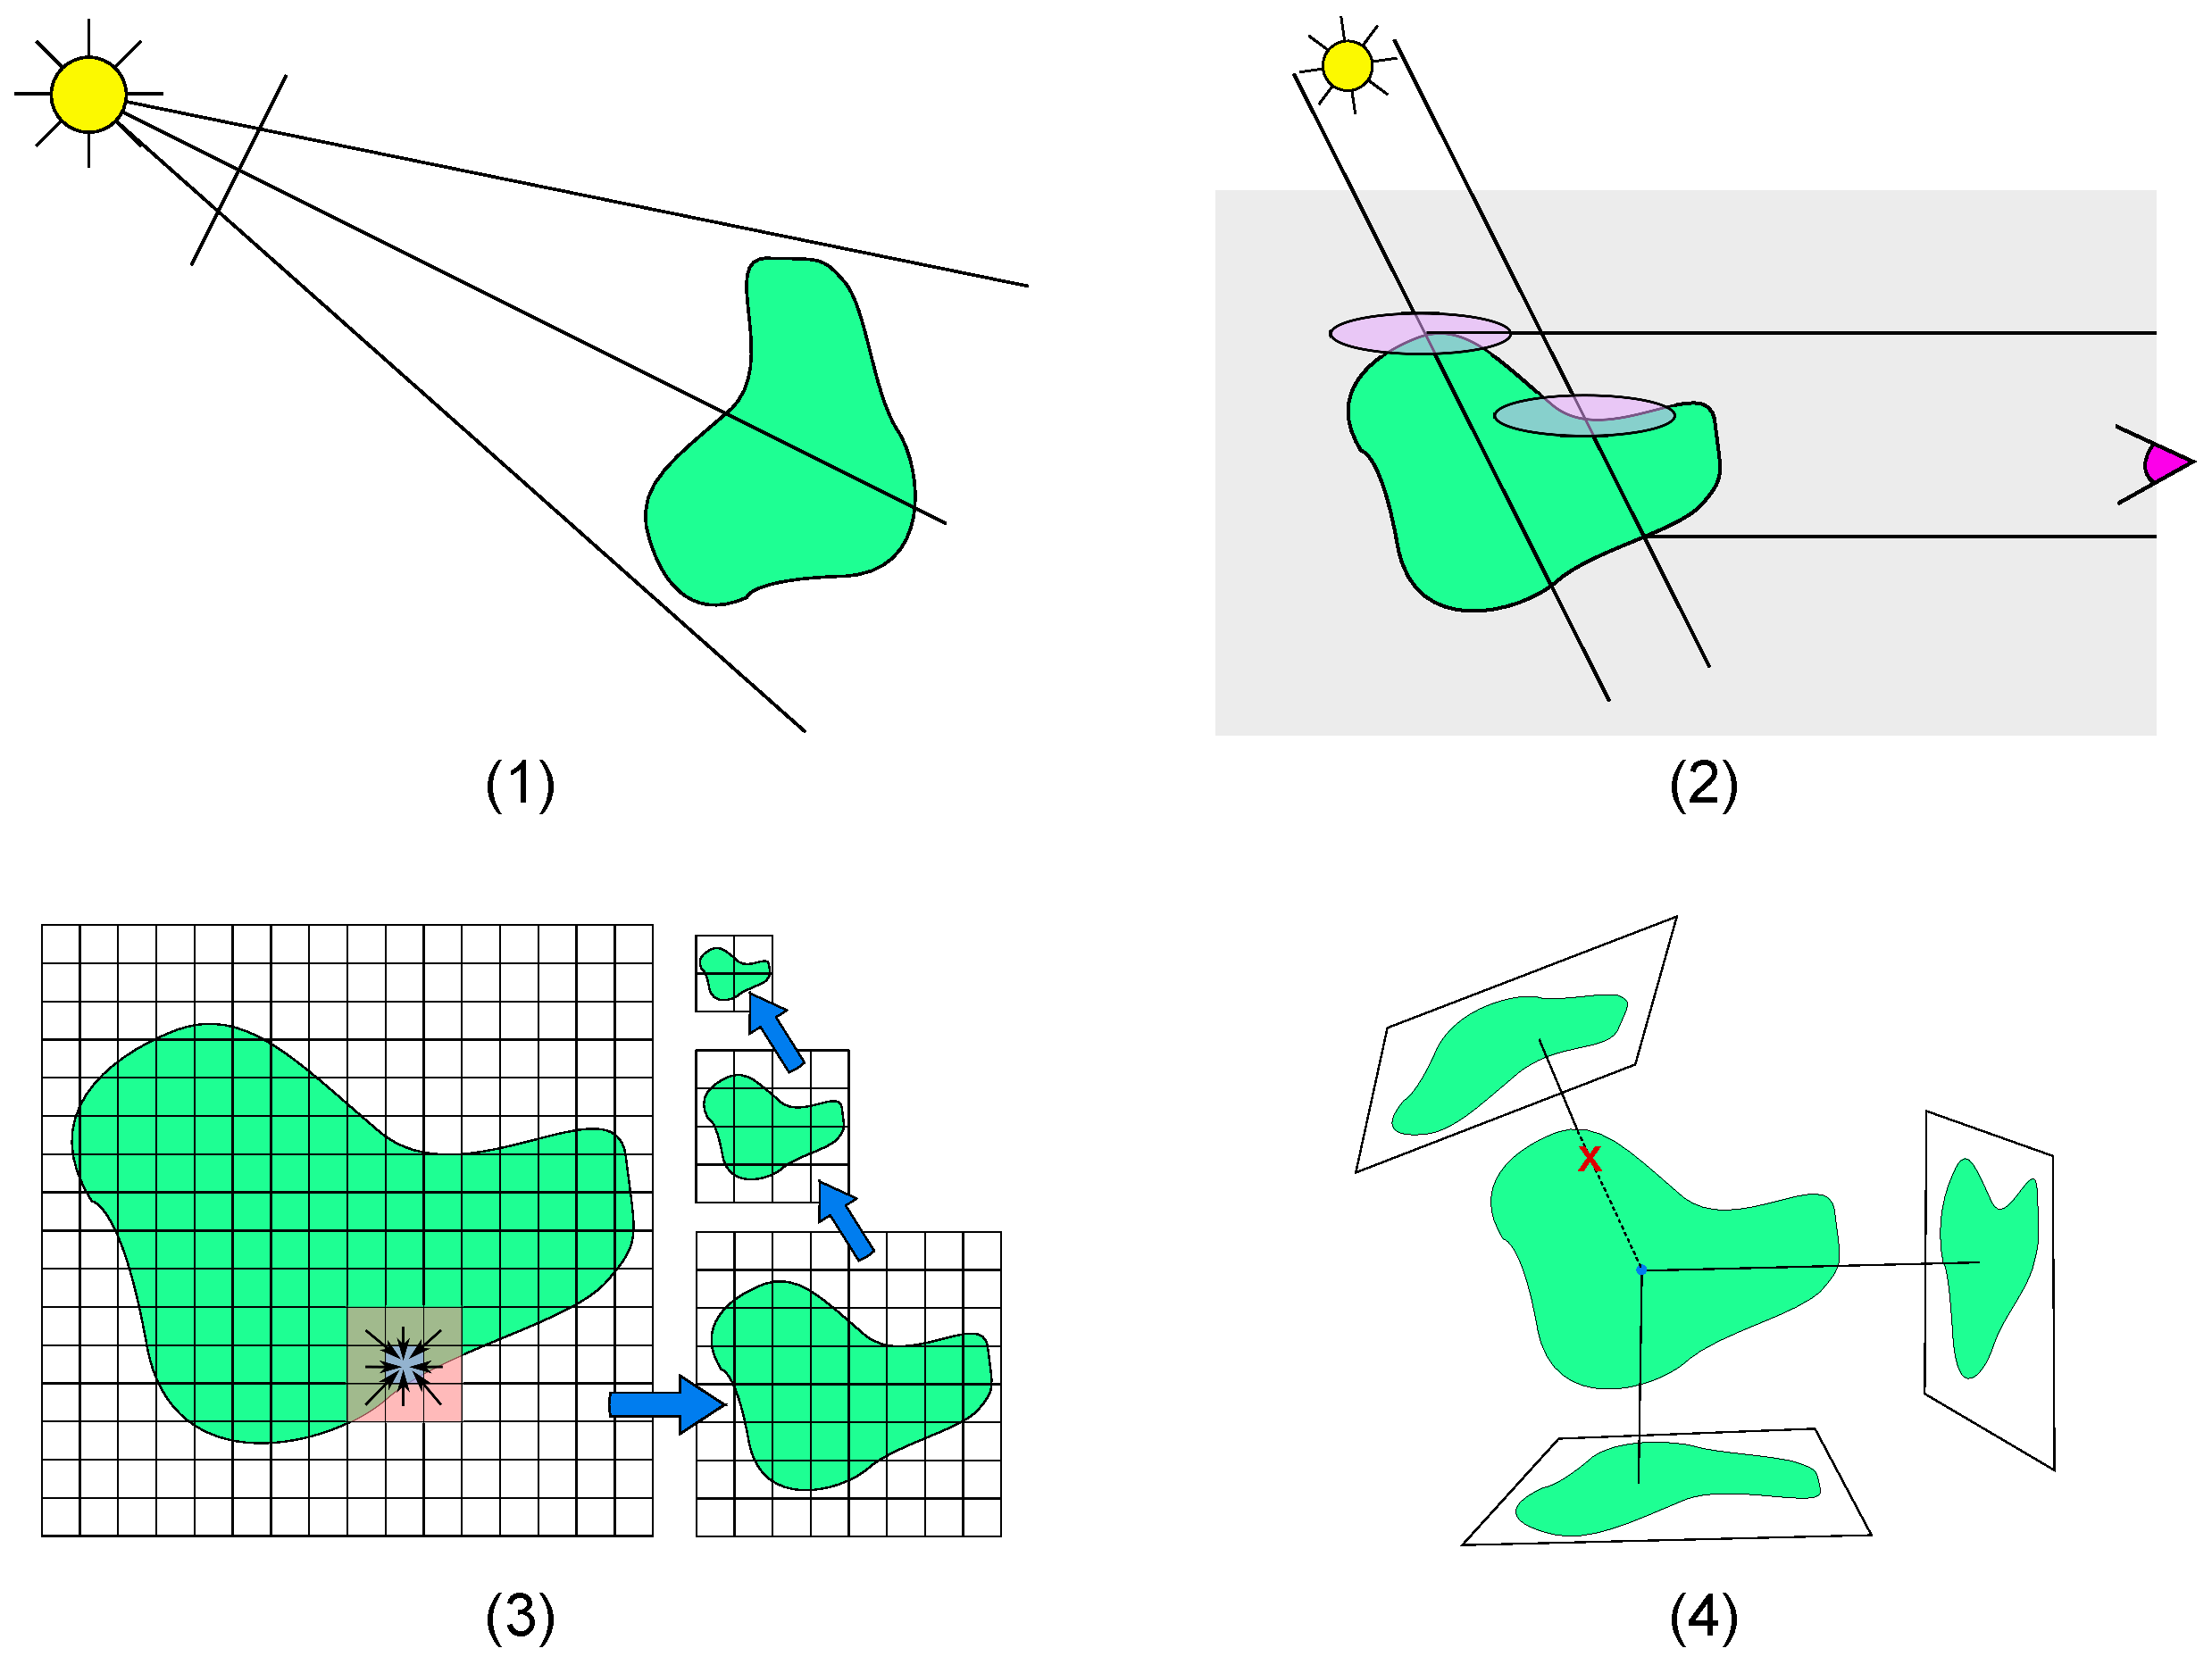
\includegraphics[scale = 0.8]{./images/combination4.eps} 
\fcaption{The various steps of the method.}
\end{center}


\textbf{Pass 3} 
\\
We generate mipmaps from the render in the previous step, applying a custom edge-preserving bilateral filter.  
\\
\textbf{Pass 4} 
\\
We render the final model using the information stored in the various layers. We sample the textures in a similar way as in shadow mapping, using a custom light world matrix that is unique per layer. In the initial frames, in order to eliminate high frequency noise, we set a high minimum mipmap level is used in order to blur the result. And make it less noticeable to the user. 

The final constants are then multiplied and averaged on the numbered of passed frames.

\csection{Results}
As we can see from the following figure, the method at convergence gives a smooth an pleasant result, in accordance with \cite{IMM2013-06646}. During the evolution to convergence, we can see that the result is quite noisy, but the filtered mipmaps remove most of the high frequency noise. We can see that some of the details in the final image are missing, but the result is good enough to trick the observer's eye. Regarding the performance, preliminary results give a rendering time of 50 milliseconds per frame on a high-end modern GPU.

\begin{center}
\includegraphics[scale = 1.3]{./images/jep} 
\fcaption{Stanford Dragon after convergence (100 frames). Scattering parameters for marble. }
\end{center}

\begin{center}
		\begin{tabular}{ccc}
			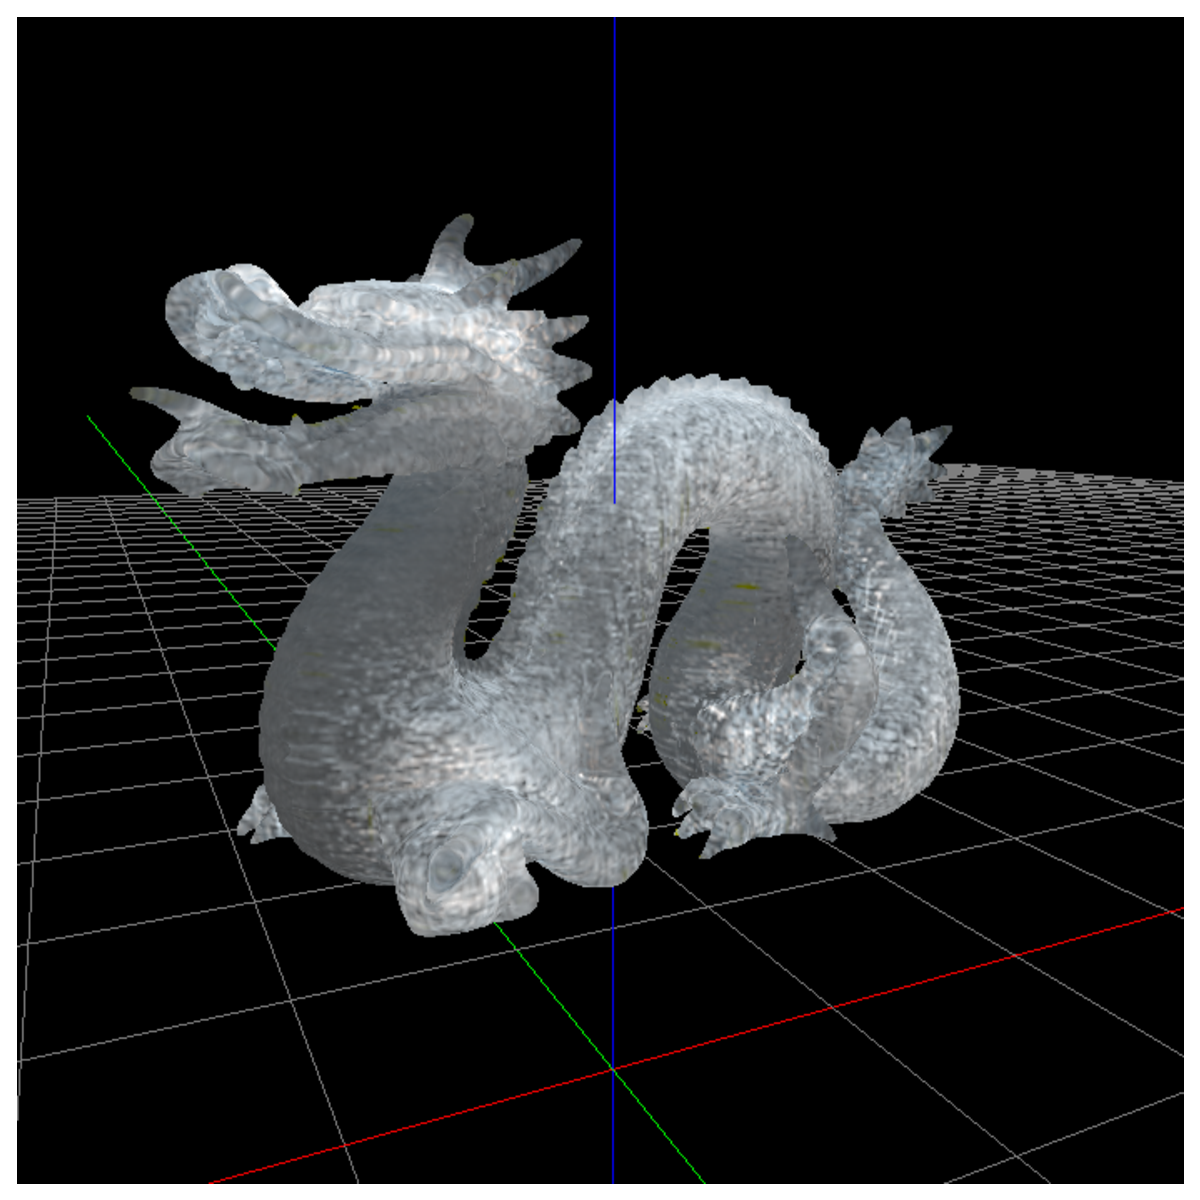
\includegraphics[width=0.33\linewidth]{./images/j1.eps}&
      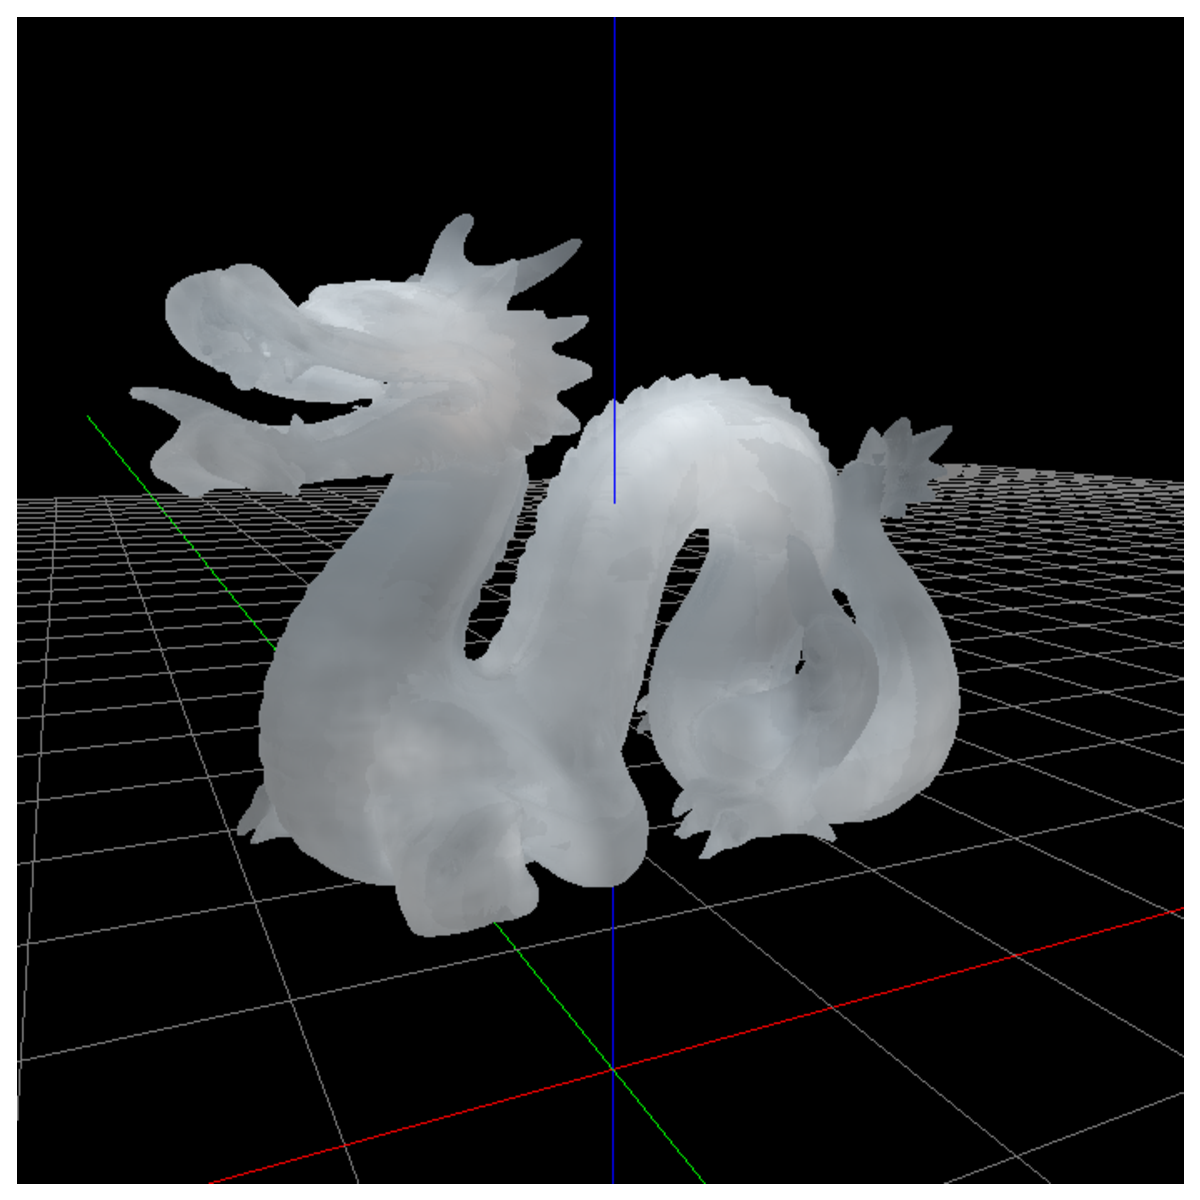
\includegraphics[width=0.33\linewidth]{./images/j2.eps} & 
      \includegraphics[width=0.33\linewidth]{./images/jep.eps} \\
																																								   
%			\includegraphics[scale = 0.9, viewport = 10 30 240 450, clip]{./images/timeComparison.pdf} &
%			\includegraphics[scale = 0.9, viewport = 10 30 240 450, clip]{./images/timeComparison_speedup.pdf}
		{\small Accumulated 5 frames, without mipmaps }&	  {\small Accumulated 5 frames, with mipmaps} & {\small Convergence (100 frames)} %\vspace{-0.5cm}
\end{tabular}
\end{center}
\fcaption{Improvement from the custom mipmaps: we can see that the filtering greatly improves the quality of the image.}
\csection{Future work}


Next steps that I would like to take in the domain of \textit{quality}:
\begin{itemize}
	\item Position the cameras accurately in order to cover the whole model (not trivial)
	\item Investigate time and sampling patterns that may help a faster convergence. 
	\item Multiple lights and introduction of point and environment lights.
\end{itemize}
\csection{References}
%
\vspace{-3cm}
\bibliographystyle{is-unsrt}
%\footnotesize{
\bibliography{./mlbib}
%}
%
\end{multicols}
%
\end{poster}
%
\end{document}
